% !TeX spellcheck = hu_HU
% !TeX encoding = UTF-8
% !TeX program = xelatex
%----------------------------------------------------------------------------
\chapter{A sorbuffer modul megvalósítása}
%----------------------------------------------------------------------------

Eddig úgy működtettem a test benchet a bilineáris filterhez, hogy a bemeneti képet (amit .raw fájlformátumban használtam, annak érdekében hogy pusztán csak a pixel adatokat tartalmazza, és egyéb header információkat ne) beolvastam egy tömbbe, és amikor a filter kért egy pixel értéket, azt csak szimplán kiindexeltem ebből a tömbből a kívánt sor és oszlop alapján. 
Ez a megoldás tesztelésre jó, de annak érdekében hogy a modul videó folyamot tudjon feldolgozni, ennél robosztusabb megoldásra van szükség. Éppen ezért megalkottam egy sorbuffer modult, aminek az a feladata, hogy eltárolja blokk-ram-okba azokat a sorokat amiket a filter éppen használ (a bilineáris filter esetén egyszerre csak 4 sort használ a szűrő, de polyphase esetén akár 4-et is használhat egyszerre), és ezekből a sorokból pedig már a megfelelő oszlopok pixeleit egyszerűen vissza lehet adni a filter számára.

Továbbá azért fontos még ez a sorbuffer modul, mert majd a továbbiakban, a bejövő video streamet és ezt a sorbuffer modult valamilyen axi interface-el fogom összekapcsolni, amivel a sorbuffer egyszerre tudja írni a blokk ramokat a bejövő video streamből, és közben a filterek számára a megfelelő pixelek értékeit pedig ki tudja adni.

\subsection{Blokkvázlat}

Tekintsük át a sorbuffer magas szintű működését először. Az architektúra blokkvázlata az \ref{pic:sorbuffer} ábrán látható. Mivel a bilineáris szűrő 2 bemeneti sor-t használ egyszerre, ezért ebben az esetben elegendő 4 sornyi blokkramot fenntartani a bufferben. 2 sornyi blokkramból párhuzamosan kiolvassuk a megfelelő oszlopok pixeleinek értékeit, és a maradék 2-be (vagy csak 1 be, vagy 0 ba, erről később) pedig beírjuk a filter által következőleg használt 2 sor értékeit. Tehát egy 2x-es kicsinyítés esetén, a kimeneti kép első sorához a bemeneti kép első két sorát olvassuk a blokkramokból, és közben a bemeneti kép következő 2 sor pixelértékeivel töltjük fel a másik 2 blokkramot, hiszen a kimeneti kép következő sorához, újabb 2 sorra van szükség.

\begin{figure}[!ht]
	\centering
	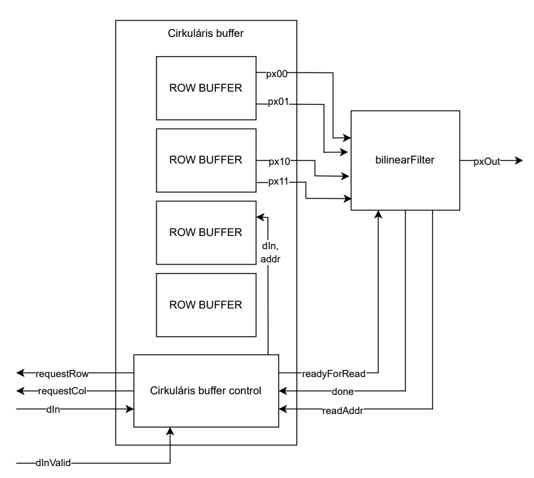
\includegraphics[width=120mm, keepaspectratio]{figures/sorbuffer.png}
	\caption{A sorbuffer architektúrája} 
	\label{pic:sorbuffer}
\end{figure}
\newpage

A működés egy cirkuláris bufferre épül, melyben $2^n$ db blokkram tud elhelyezkedni. Ha a filter $k$ sort használ használ fel a kimeneti pixel meghatározásához, akkor legalább $2k$ blokkramra van szükség a modulban annak érdekében, hogy a legrosszabb esetben is képes legyen a modul egyszerre írni a bejövő adatokat blokkramokba, és a filter tudja olvasni a számára szükséges adatokat. 

Tehát mivel a bilineáris filter 2 sort használ, ezért annál $n=2$, és mivel a polyphase filter pl 4 sort használhat, ezért ott $n=3$.

A cirkuláris bufferben van egy writePointer, és egy ReadPointer. Amikor egy újabb sort beolvasunk, akkor a writePointert inkrementáljuk, és egy újabb blokkramba olvassuk be a bemeneti adatokat. Amikor újabb sort akarunk koilvasni, akkor pedig a readPointert inkrementáljuk eggyel. Ha túlcsordulna bármelyik pointer, semmi probléma nincsen, a következő blokkram az akkor a 0. lesz akár olvasásról akár írásról van szó. Ezek a pointerek kezelik azt, hogy melyik blokkramból olvasunk ki és melyikbe írunk. Egyszerre csak egy blokkramba írunk, ugyanakkor mivel a bilineáris filternek 2 sorra van szükségea működésre, ezért egyszerre 2 sorból olvasunk. Ez nem probléma, hiszen abból a sorból sosem fogunk olvasni, amelyikbe éppen írunk, vagyis amelyikre éppen a writePointer mutat. Azonban ez az eset a kép legvégén megtörténhet, amikor is már nem olvasunk be több sort, és az utolsó sort olvassuk ki. Ekkor a write pointer és a read pointer ugyan arra a blokkramra mutat. Azonban ilyenkor tudjuk, hogy olvasni akarunk, ezért egy extra változó bevezetésével (forceRead) megoldhatjuk azt a problémát, hogy olvasás valósuljon meg a megadott címre, és ne pedig olvasás. 

Ezen kívül az olvasáskor mindig 2 sort kell olvasnunk, azt amelyikre a readpointer mutat, és a következőt. Ezeken felül az oszlopokból mindig azt kell olvasni amelyiket a bilineáris filter kér, (requestCol), és a következőt. Az alábbi kódrészlet azt mutatja be, hogy ez az írás olvasás logika hogyan van megvalósítva.

\begin{minted}{verilog}
wire [DATA_WIDTH-1:0] ramDataOutA [2**BUFFER_SIZE-1:0];
wire [DATA_WIDTH-1:0] ramDataOutB [2**BUFFER_SIZE-1:0];
//generating the RAM blocks 
generate
genvar i;
for(i = 0; i < 2**BUFFER_SIZE; i = i + 1)
begin : ram_generate
ram #(
.DATA_WIDTH(DATA_WIDTH),
.ADDRESS_WIDTH(ORIG_X_SIZE)
) ram_inst_i(
.clk( clk ),

//Port A is written to as well as read from. 
//When writing, this port cannot be read from.
.addrA( ((writeSelect == i) && !forceRead && writeEnable) ? requestCol : readAddress ),
.dataA( writeData ),													
.weA( ((writeSelect == i) && !forceRead) ? writeEnable : 1'b0 ),
.outA( ramDataOutA[i] ),

//portB is only read from, we are reading the next pixel 
.addrB( readAddress + 1'b1 ),
.dataB( writeData ),
.weB( 1'b0 ),
.outB( ramDataOutB[i] )
);
end
endgenerate

//Select which ram to read from
wire [BUFFER_SIZE-1:0]	readSelect0 = readSelect;
wire [BUFFER_SIZE-1:0]	readSelect1 = readSelect+1;

//Steer the output data to the right ports
assign readData00 = ramDataOutA[readSelect0];
assign readData01 = ramDataOutB[readSelect0];
assign readData10 = ramDataOutA[readSelect1];
assign readData11 = ramDataOutB[readSelect1];
\end{minted}

Mivel a ram egységek amiket példányosítottunk dual port ramok, ezért meg tudjuk csinálni hogy egyszerre 2 pixelt olvasunk ki belőlük. Éppen ezért a második porton csak olvasunk, és az első porton van lekezelve az írás logikája.

\subsection{Állapotgép}

A sorbuffer modulnak kicsit bonyolultabb állapotgépe van mint a bilinear filter modulnak. Az alapvető gondolat a működése mögött az az, hogy ebben a modulban is jelen van egy számláló, ami a bemeneti képen levő pixel helyzetét számolja (vagyis csak a sorának a helyzetét). Ha ennek a számlálónak az értéke nem billen át egy következő egész számra, (tehát pl 0-ról 0.6666-ra vált az értéke) akkor nem kell újabb sort beolvasnunk ahhoz, hogy a filter számára új adat elérhető legyen, hiszen ugyan azt a két sort fogja használni a következő kimeneti sor meghatározásához, mint amit eddig használt. 

Azonban ha a számláló értéke átbillen egy következő egészre (pl 0.666-ról 1.333-ra) akkor a filter következő kimeneti sorának az előállításához már a 0. bemeneti sorra nincs szükség, viszont a 2. bemeneti sorra igen. Ekkor beolvassuk az újabb bemeneti sort, és amikor végez a filter a jelenlegi sor feldolgozásával, a read pointert 1-el fogjuk növelni, ezáltal az outputra az 1. és 2. sor pixelei fognak majd kerülni olvasáskor.

Az utolsó eset, ha a sorszámláló értéke több mint 1 egésszel nőtt. Ekkor lényegtelen hogy mennyi egésszel nőtt az értéke, lehet az 2 is vagy akár 5, mindenképpen 2 új sort kell beolvasnunk, és a read pointert a következő sor feldolgozásánál 2 vel kell növelnünk, hogy a filter számára a 2 frissen beolvasott sor legyen elérhető.

Most, hogy megértettük a működés alapelvét, tekintsük meg az állapotgépet, és nézzük meg mi történik az egyes állapotokban.

\begin{figure}[!ht]
	\centering
	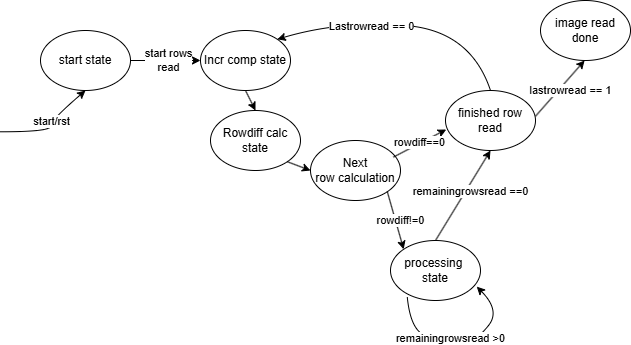
\includegraphics[width=120mm, keepaspectratio]{figures/sorbuffer_allapotgep.png}
	\caption{A sorbuffer állapotgépe} 
	\label{pic:sorbuffer_allapotgep}
\end{figure}

\begin{itemize}
	\item Start state: itt beolvasásra kerül az első 2 sor, hiszen azt mindenképpen be kell olvasni, ez lesz az első 2 sor amit a filter felhasznál. Amint ez befejeződött, a modul high-ra állítja a readyForRead outputot 1 órajelig, ezzel jelezve a filter modulnak hogy megkezdheti az első sor feldolgozását.
	\item Incr comp state: Kiszámoljuk a következő sornak az értékét, és az előzőnek az értékét elmentjük egy másik reg-be.
	\item Rowdiff calc state: Az incr comp state ben kiszámolt és elmentett két regiszter értékének a különbségét vesszük, és meghatározzuk, hogy mennyi egész szám került átlépésre a két sor között. Ezt az értéket a rowDiff regiszterbe mentjük.
	\item Next row calculation state: Itt az alapján hogy mi volt az előbb meghatározott rowdiff értéke, a következőket csinálhatjuk:
	\begin{itemize}
		\item rowDiff==0 esetén a következő sorok ugyan azok lesznek amik jelenleg is el vannak mentve, tehát nincs teendő, a finished row read state be ugrunk.
		\item rowDiff < NUMROWSTOSTORE mivel a bilineáris filter esetén 2 sort kell elmentenünk, ezért ha a rowDiff az ennél kevesebb (de 0 nál több, tehát 1), akkor a write pointert  eggyel növeljük, elmentjük hogy eggyel kevesebb sort kell beolvasnunk (bilineáris filter esetén ez 0 lesz), a remainingRowReads regiszterbe, és azt is elmentjük hogy mennyivel kell majd inkrementálni a read pointert, amikor a filter befejezte az előző sorok feldolgozását. Processing state-be ugrunk.
		\item a harmadik esetben 2 vel kell növelni (vagyis annyival amennyi sort eltárolunk a filter működéséhez) a write pointert, és azt is eltároljuk, hogy 2 vel kell megnövelni majd a read pointert. Ezen kívül azt is eltároljuk, hogy mennyi sor olvasása van még hátra (ez a bilineáris filter esetén 1 lesz). Processing state-be ugrunk.
	\end{itemize}
	\item Processing state: hasonlóan a start state hez, addig olvasunk be sorokat, ameddig be nem olvastuk a megfelelő mennyiségű sorokat, amit az előző state ben meghatároztunk. Ezek után a finished row state be ugrunk.
	\item finished row state: ha itt vagyunk, az azt jelenti hogy egy sort beolvastunk. Ez tehát azt jelenti, hogy a filter számára elérhetőek a következő sorok amiket használ, attól függetlenül, hogy azok ugyan azok-e vagy különbözőek attól, amiket most használ. Ebben a state ben ha a filter jelez hogy elkészült a sorok feldolgozásával, akkor újra visszaugrunk az incremenet compute state be, és előröl elkezdődik a folyamat, beolvassuk a filter számára szükséges következő sorokat. Ha azonban a kép végére értünk, akkor a finished image state be ugrunk, és a force read regisztert magasba rakjuk, hogy az utolsó sorból is ki tujda olvasni a filter a pixel értékeket.
	\item finished image state: készen vagyunk, beolvastuk az egész bemeneti képet. Resettel vagy start inputtal újra a start state be hozható az állapotgép
\end{itemize}

\subsection{Sorbuffer modul bővítése}

Ugyan a sorbuffer modult főként csak a bilineáris filterrel tudtam tesztelni, megpróbáltam egy olyan architektúrát létrehozni, amivel a polyphase filter esetén is használható lesz. Ugyan minden ilyen fejlesztést még nem sikerült implementálnom, de már gondolkodtam rajta hogy miket kellene változtatni. 
\begin{itemize}
	\item Nem lesz elég a filternek az oszlopot megadni hogy melyik pixeleet kéri a bemeneti képből, a sorok is kelleni fognak, hacsak nem bővítem a sorbuffer modul kimeneteit arra, hogy 4 sornak a pixeleit tudja egyszerre kiadni a kimenetre
	\item polyphase filternél nem azt kell majd itt számon tartani, hogy mi a kimeneti pixel bemeneti képén velő helye, hanem azt, hogy melyik sorban kezdődik a filter ablaka. Erre már előre létrehoztam egy numrowstostore parameter-t, aminek a segítségével ez számítható lesz.
\end{itemize}

\chapter{Eredmények, a projekt helyzete}

A projekt jelenlegi állása szerinte képes a bilineáris filterrel és a sorbufferekkel kiegészített modul segítségével tetszőlegesen átméretezni képeket. Mindkét modulhoz (sorbuffer modul, és bilineáris filter modul) készült testbench, amikkel azok működése ellenőrizhetővé vált. Ezen kívül elkészült egy harmadik testbench is, amiben a két modul integrálva van, és egymáshoz van csatlakoztatva. Néhány próba kép a \ref{sec:kepek} fejezetben található, ahol az eredeti 256x256 lena képet nagyítottam fel, majd egy tetszőleges méretűre méreteztem át.

A polyphase filter idő szűkében sajnos nem került még megvalósításra, még jelenleg fejlesztés alatt van, de mivel az irodalomkutatás része már megvan, ezért azta jövőben jóval egyszerűbb lesz megvalósítani, mint akár a félév elején az egyszerűbb bilineáris filtert. Ezt lehet az első továbbfejlesztésnek nevezni.

Ezen kívül a projekt jelenleg csak standalone képeket tud átméretezni, video folyamot nem, úgyhogy ezt a fejlesztést, hogy valamilyen axi interface-t csatlakoztatunk a sorbuffer modulhoz, és egy bemeneti video streamet juttatunk el annak, lehetne a második nagyobb fejlesztésnek is nevezni.

Harmadikként pedig a sorbuffer modul kisebb átdolgozsára szorul, hogy a polyphase filterrel is működni tudjon, de ezt már annak a fejezetében is említettem. A fejlesztés során próbáltam gondolni arra, hogy kicsit általánosabban működjön a sorbuffer modul, de mivel nem volt polyphase filter modulom elkészülve, amivel tesztelni tudtam volna, ezért ezt nem is tudtam 100\% ban így fejleszteni.

A projekt során rengeteget tanultam, mind a verilog nyelvből, mind FPGA működéséről, (hiszen ezekkel most találkoztam először) mind pedig általános képfeldolgozásról. Több külső eszközt kellett használnom hogy ellenőrizzem az eredményeim, ilyenek pl az IrfanView a .raw képek megtekintésére, vagy az ImHex hex editor, ahol a képeket pixel érték szinten tudtam vizsgálni. Ezen kívül segéd python scripteket is kellett írnom a modul teszteléséhez pl a scale factor megállapításához. A projekt forráskódja megtalálható a saját Githubomon, az alábbi linken: \url{https://github.com/NuunMoon/FPGA_scaler}